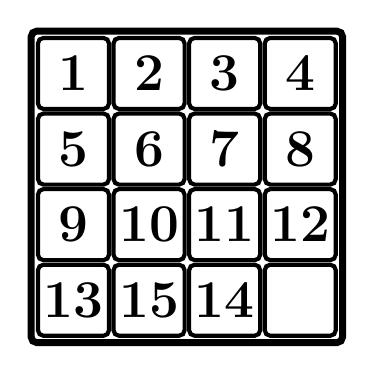
\begin{tikzpicture}[
    scale=0.60,
    transform shape,
    x=1.6cm,
    y=1.6cm,
    tile/.style={
        draw=black,
        fill=white,
        line width=1.5pt,
        rounded corners=2pt
    },
    every node/.style={
    font=\fontsize{24.88}{30}\selectfont\bfseries,
    scale=1.28617
    }
]

% Outer frame
\draw[
    draw=black,
    fill=white,
    line width=2.5pt,
    rounded corners=2pt
] (-0.06,-0.06) rectangle (4.06,4.06);

% Tiles listed from left to right, top to bottom.
% The final empty entry produces the blank square.
\foreach \value [count=\i from 0] in {
    1,2,3,4,
    5,6,7,8,
    9,10,11,12,
    13,15,14,{}
}{
    \pgfmathtruncatemacro{\col}{mod(\i,4)}
    \pgfmathtruncatemacro{\row}{3-floor(\i/4)}

    \draw[tile]
        ({\col+0.03},{\row+0.03})
        rectangle
        ({\col+0.97},{\row+0.97});

    \node at ({\col+0.5},{\row+0.5}) {\value};
}
\end{tikzpicture}
